\begin{frame}{$\DPLL$ algorithms}

    $\varphi \coloneqq (x \lor \neg{y} \land z) \land (\neg{x} \lor w \land z \land s) \land
    (\neg{x} \lor \neg{z} \lor s) \land \dots$

    \pause
    \begin{center}
    	\onslide<1->{
   	\tikzstyle{vertex2} = [opacity = 0]
   	\tikzstyle{vertex3} = [opacity = 0]
    \tikzstyle{vertex4} = [opacity = 0]
   	\tikzstyle{vertex5} = [opacity = 0]
    \tikzstyle{vertex9} = [opacity = 0]
    \tikzstyle{vertex11} = [opacity = 0]
}
\only<2->{\tikzstyle{vertex2} = [opacity = 1]}
\only<3->{\tikzstyle{vertex3} = [opacity = 1]}
\only<4->{\tikzstyle{vertex4} = [opacity = 1]}
\only<5->{
  	\tikzstyle{vertex5} = [opacity = 1]
    \tikzstyle{vertex9} = [opacity = 1]
}

\tikzstyle{end} = [circle, minimum size = 0.6cm, draw = black, inner sep = 0.1pt]
            
\tikzstyle{level 1} = [draw = black, level distance = 1.5cm, sibling distance = 5cm]
\tikzstyle{level 2} = [sibling distance = 2cm]
    
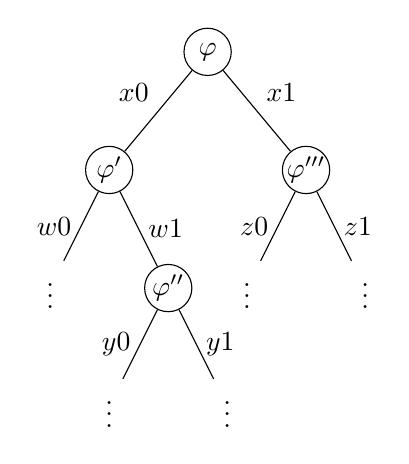
\begin{tikzpicture}[label distance=8mm]
	\node [end] (z){$\varphi$}
		child [vertex2] {
    		node [end] (b) {$\varphi'$}
			child [vertex3]{
	           	node {$\vdots$}
                edge from parent
	  	        node[left] {$w \coloneqq 0$}
            }
		    child [vertex4]{
            	node[end] {$\varphi''$}
            	child [vertex4]{
            	   	node {$\vdots$}
            		edge from parent
	  	        	node[left] {$y \coloneqq 0$}
                }
                child [vertex4]{
            	   	node {$\vdots$}
            		edge from parent
	  	        	node[right] {$y \coloneqq 1$}
            	}
                edge from parent
	   	        node[right] {$w \coloneqq 1$}
            }
           	edge from parent
            node[above left] {$x \coloneqq 0$}
        }
        child [vertex5] {
        	node [end] (c) {$\varphi'''$}
           	child [vertex9]{
               	node {$\vdots$}
                edge from parent
	            node[left] {$z \coloneqq 0$}
            }
		    child [vertex9]{
               	node {$\vdots$}
                edge from parent
	            node[right] {$z \coloneqq 1$}
            }
            edge from parent
	   	    node[above right] {$x \coloneqq 1$}
        };
\end{tikzpicture}    
    \end{center}

    \vspace{0.1cm}
        
	\pause
    \pause
    \pause
    \pause

    Can we estimate running time of this algorithm?

\end{frame}

\begin{frame}{Canonical search problem $\Search_{\varphi}$ (Lov{\'{a}}sz et al. 1994)}
    
    $\varphi(x, y)$ is an unsatisfiable CNF formula:
    \begin{itemize}
        \item Alice receives an assignment to the variables $x$, Bob receives an assignment to the
            variables $y$;
        \item goal is to find a clause $C \in \varphi$ that is unsatisfied by this assignment.
    \end{itemize}

    \pause

    \begin{block}{Beame, Pitassi, Segerlind 06; Huynh, Nordstr{\"{o}}m 12; G{\"{o}}{\"{o}}s, Pitassi 14}
        There is a CNF formula $\varphi$ on $n$ variables such that:
        $$\RCC(\Search_{\varphi}) \ge \RCC(\DISJ_{\frac{n}{\log n}}) = \Omega\left( \frac{n}{\log n} \right).$$
    \end{block}

    \begin{block}{Lov{\'{a}}sz et al. 1994}
        Running time of $\DPLL$ on formula $\varphi$ algorithm is at least $2^{\DCC(\Search_{\varphi})}$.
    \end{block}
\end{frame}

\begin{frame}{Lower bound on $\DPLL$}

    \begin{block}{Lov{\'{a}}sz et al. 1994}
        Running time of $\DPLL$ on formula $\varphi$ algorithm is at least $2^{\DCC(\Search_{\varphi})}$.
    \end{block}

    \begin{minipage}{0.54\linewidth}
        \begin{enumerate}
            \item<2-> Pick a subtree $T'$ such that: $\frac{1}{3}|T| \le |T'| \le \frac{1}{3}|T|$.
            \item<4-> Check whether we reach this subtree. Two bits of communication.
            \item<6-> If ``yes'', run algorithm for $T'$.
            \item<7-> If ``no'', run algorithm for $T \setminus T'$.
        \end{enumerate}
    \end{minipage}
    \begin{minipage}{0.45\linewidth}
        \begin{center}
            \tikzstyle{subtree} = [opacity = 0]
\only<3->{\tikzstyle{subtree} = [opacity = 1]}

\tikzstyle{norm} = [semithick, draw = black]
\tikzstyle{acedge} = [black]
\only<5-7>{
    \tikzstyle{acedge} = [
        draw = LEIorange!80, 
        ultra thick]
}


\tikzstyle{end} = [draw, circle, minimum size = 0.6cm, inner sep = 0.1pt]

            
\tikzstyle{level 1} = [level distance = 1.5cm, sibling distance = 2.5cm]
\tikzstyle{level 2} = [sibling distance = 1.5cm]
\tikzstyle{level 3} = [sibling distance = 1.5cm]
    
\begin{tikzpicture}[label distance = 8mm]
    \node[end, acedge] (z) at (0, 0) {$\varphi$}
        child[end]{
            node[end, acedge] {$\varphi'$}
            child[end]{
                node {$\vdots$}
                edge from parent[norm]
	  	        node[above left] {$w \coloneqq 0$}
            }
		    child[end]{
            	node[end] (o) {$\varphi''$}
            	child[end]{
            	   	node {$\vdots$}
            		edge from parent[norm]
	  	        	node[above left] (a) {$y \coloneqq 0$}
                }
                child[end]{
            	   	node {$\vdots$}
            		edge from parent[norm]
	  	        	node[above right] (b) {$y \coloneqq 1$}
            	}
                edge from parent
                node[above right, black] {$w \coloneqq 1$}
            }
           	edge from parent[acedge]
            node[above left, black] {$x \coloneqq 0$}
        }
        child[end]{
            node[end] (c) {$\varphi'''$}
            child[end]{
               	node {$\vdots$}
                edge from parent[norm]
	            node[above left] {$z \coloneqq 0$}
            }
		    child[end]{
               	node {$\vdots$}
                edge from parent[norm]
	            node[above right] {$z \coloneqq 1$}
            }
            edge from parent[norm]
	   	    node[above right] {$x \coloneqq 1$}
        };

        \begin{scope}[on background layer]
            \draw[subtree, ultra thick, orange!25, fill = orange!10, rounded corners = 0.8cm]
                ($(a) + (225:2.12)$) -- ($(o) + (0, 1)$) --
                ($(b) + (-45:2.12)$) node[shift = {(-0.8, 0.3)}, black] {$T'$} -- cycle;
        \end{scope}
\end{tikzpicture}
        \end{center}
    \end{minipage}

    \vspace{0.1cm}
        
	\pause
    \pause
    \pause
    \pause
    \pause
    \pause
    \pause
    
    \vspace{0.1cm}

    We need at most $\log |T|$ recursive calls.

\end{frame}